\section{Introducción Teórica}

\subsection{El Problema y su representación}


\begin{wrapfigure}{r}{0.5\textwidth}
  \vspace{-20pt}
  \begin{center}
    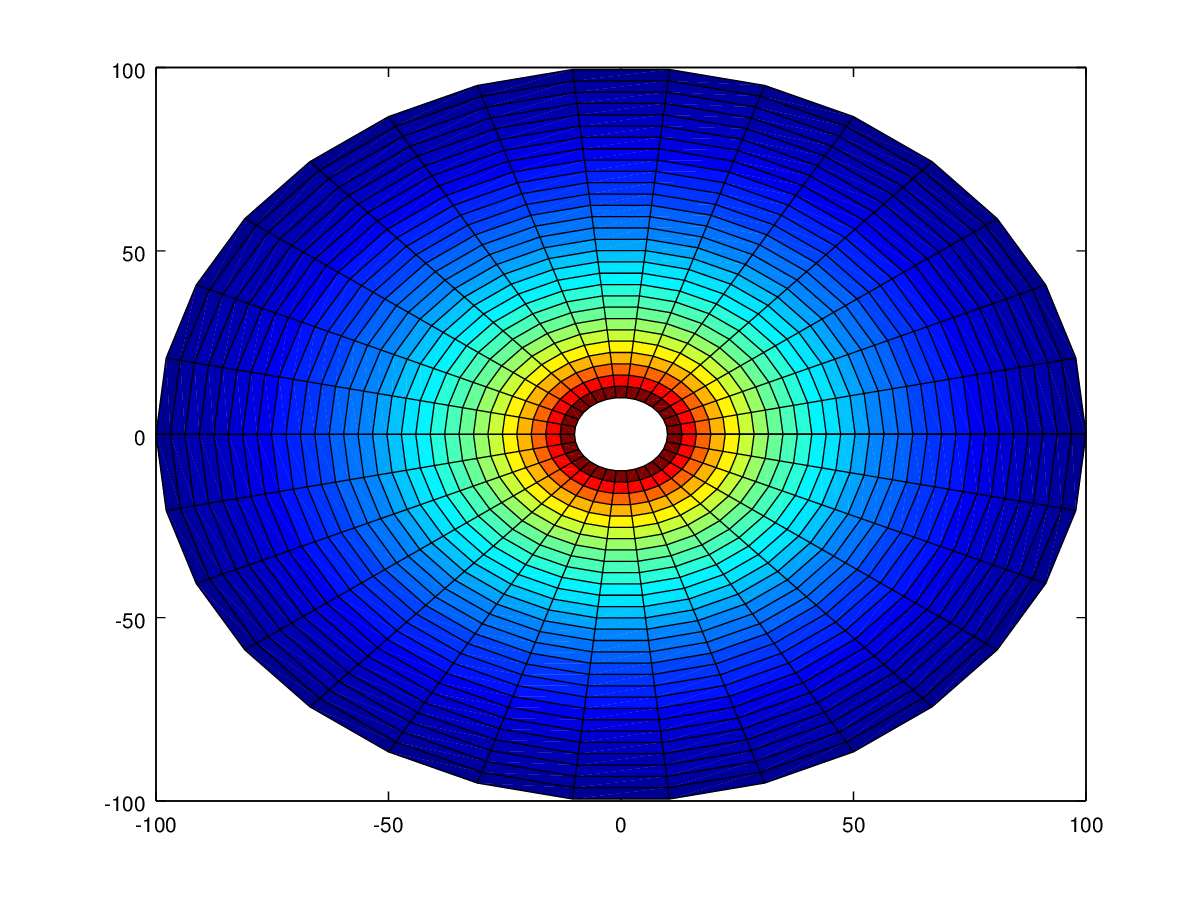
\includegraphics[scale= 0.4]{../hornoEjemplo.png}
  \end{center}
  \vspace{-20pt}
  \caption{Temperatura de un horno.}
  \vspace{-10pt}
  \label{fig:corteHorno}
\end{wrapfigure}

Queremos medir temperaturas de un horno industrial cilíndrico utilizado para fundir metales. Dicho horno tiene una pared interior y una exterior, cuyas temperaturas (la de las paredes) son conocidas en determinados puntos. Sabemos que la pared exterior tiene un límite de temperatura máxima, y nuestro objetivo es determinar si dicha temperatura máxima es alcanzada o no. Para ello, buscamos los puntos en el horno cuya temperatura alcance los 500 grados celcius.  Si esta temperatura es cercana al borde exterior se corre peligro por parte de los trabajadores de una hipotética fábrica que utilice dicho horno.




El problema se reduce a determinar dónde se encuentra la isoterma 500 en un círculo, como el que se ve en la figura, que representa un corte del horno. Las pared externa del horno es la circunferencia, y la pared interna es la circunferencia del circulo interno.



\subsection{Solucionando el problema}

Usando las herramientas aprendidas en la materia (sistemas de ecuaciones lineales, y sus métodos de solución, como Eliminación Gaussiana o factorización LU) queremos representar las temperaturas en distintos puntos del horno como incógnitas de un sistema lineal de ecuaciones que resolveremos.
 Para esto vamos a discretizar el espacio para tener finitas incógnitas, y vamos a usar ecuaciones de calor y la información de las temperaturas en finitos puntos de las paredes y así armar la matriz con los coeficientes del sistema.\\



\begin{wrapfigure}{r}{0.5\textwidth}
  \vspace{-20pt}
  \begin{center}
    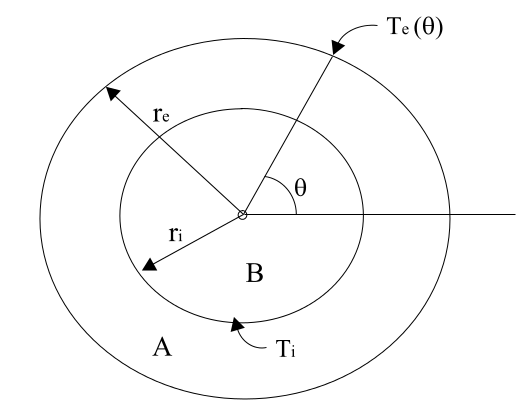
\includegraphics[scale= 0.4]{../Horno.png}
  \end{center}
  \vspace{-20pt}
  \caption{Corte del horno.}
  \vspace{-10pt}
  \label{fig:corteHorno}
\end{wrapfigure}


Una instancia del problema equivale a un corte del horno como se ilustra en la figura ~\ref{fig:corteHorno}. Dado que la medición de temperatura en el horno puede realizarse en infinitos puntos, discretizamos el problema fijando la ubicación de los mismos de la siguiente manera; Dividimos el horno en \textbf{\textit{n}} cantidad de ángulos de tamaño $\Delta_{\theta}$ y en \textbf{\textit{m + 1}} cantidad de radios, de tamaño $\Delta_{r}$. Analizaremos las temperaturas en los puntos donde se unen las divisiones entre ángulos y radios. Recordemos que los puntos de la pared interna y externa son dato.\\
\\


 % explicar las ecuaciones de calor




A continuación hay una breve introducción a los algoritmos conocidos y teoría que aplicamos y usamos en el trabajo.

\subsubsection{Eliminación Gaussiana}
Dada una matriz A $\in R^{nxn}$ queremos resolver el sistema $Ax = b$. El algoritmo de Eliminación Gaussiana se usa para simplificar el sistema de ecuaciones ya que produce una matriz triangular superior equivalente a la original. Esto facilita el despeje de las incógnitas con el uso de otro algoritmo llamado Backward Substitution. Las tres operaciones principales que se llevan a cabo son, suma entre filas, multiplicación de una fila por un coeficiente distinto de cero e intercambio de filas. Dichas operaciones mantienen la equivalencia.

\subsubsection{Backward Substitution}
El método Backward Substitution consiste en la obtención de los valores de las incógnitas a partir de la matriz triangulada. El método recorre cada fila de esta matriz en orden decreciente en filas. Con lo que el despeje de las incógnitas simplemente consiste en despejar el valor de la diagonal respecto al resto de los valores ya obtenidos en iteraciones anteriores.

\subsubsection{Factorización LU}
El algoritmo de Factorización LU surge ante el problema que se presenta cuando queremos resolver un sistema de ecuaciones similar a uno anteriormente resuelto. Dado el sistema de ecuaciones $Ax = b$, una vez obtenida la matriz triangulada, no queda registro alguno de las operaciones realizadas. Si estas fueran guardadas de alguna manera, podríamos reflejarlas en $b^{*}$  para cada nuevo sistema $Ax = b^{*}$. Repetir E.G. tendría un costo adicional de $O(n^{3})$, sin embargo con la factorización LU este costo solo se tiene una sola vez.


\subsection{Bibliografía}

\begin{itemize}
\item Burden y J.D.Faires, Análisis numérico, International Thomson Editors
\item Manual de LaTeX: https://es.wikibooks.org/wiki/Manual_de_LaTeX
\end{itemize}